\documentclass{../../myassignment}
\courselabel{IN2060}
\exercisesheet{Oblig 3}{Assemblerprogrammering}

\begin{document}
	\subsection*{Del 1}
	\begin{problem}
	    Hvem er det som har ansvar for registrene, og hvilke registre, når det kalles en funksjon under ARM funksjonskallkonvensjon?

	\end{problem}

	\begin{answer}
		\texttt{R0-R3} er midertidlige variabler som blir brukt som argumenter. Disse har funskjonen som blir kalt på ansvar for. Om man trenger flere variabler en dette trenger vi en stack, og gir dermed tilgang til flere registere til en funskjon.

	\end{answer}

	\begin{problem}
	    Hva skjer med input argumentet til fib funksjonen etter at fib returnerer?

	\end{problem}
		\texttt{R0} blir brukt som return-verdien, og blir dermed slettet fra minne etter at \texttt{fib} returnerer.

	\begin{answer}

	\end{answer}

	\begin{problem}
		Hvilken endring måtte du gjøre fra Del 1 slik at programmet avsluttes riktig og hvorfor måtte dette gjøres?

	\end{problem}

	\begin{answer}
		Jeg måtte wrappe main-funskjonen i en stack for å kunne lagre den midertidlig. Etter jeg var ferdig med å printe verdiene kunne jeg tømme stacken.

	\end{answer}

	\pagebreak
	\subsection*{Del 3}

	\begin{problem}
    Undersøk den produserte Assembler koden og sammenlign med din egen kildekode fra Del 2, er det noen store forskjeller mellom det du lagde og det GCC produserer?

	\end{problem}

	\begin{answer}
	Den største forskjellen mellom koden jeg har skrevet og den maskinen har skrevet er antall ekstra kode som egentlig bare er instillinger. I tilleg bruker den flere labels og hopper en del mer mellom forskjellige punkter i koden.

	\end{answer}

	\begin{problem}
    Endre -Os til -O2, hvordan påvirker dette den produserte koden? Prøv å endre til -O3, ser du noen forandring nå?

	\end{problem}

	\begin{answer}
	Det virker som om \texttt{O2} lager en mer effektiv kode med bekostning på plass, mens \texttt{O3} lager en kode som er vanskelig å forstå. Den ser mer effektiv ut, i og med at den allerede har kalkulert \texttt{233} allerede i kompilasjonen.

	\end{answer}

	\begin{problem}
    	Hvilke argumenter er det for og i mot å bruke en kompilator sammenlignet med å skrive Assembler? Tenk spesielt på hvor mye jobb det ville være å oversette programsnuttene i Del 1, 2 og 3 til en annen prosessorarkitektur.

	\end{problem}

	\begin{answer}
		Å skrive Assembler-kode direkte er mer effektivt, men tar mye lenger tid å produsere. I tilleg er det mindre fornuftig for gjenbruk, i og med at det er ganske maskin-og-tids-avhengig kode. Det som fungerer nå vil sannsynligvis være unyttig kode om 10 år. I tillegg er kompilatorene ofte flinkere til å lage effektiv kode. Om et ledd i koden er ekstra treg kan man sjekke Assembler-koden som blir produsert av kompilatoren, og justere til målet vårt istedenfor.

	\end{answer}

	\pagebreak
	\subsection*{Del 4}
	\begin{problem}

	    Oversett 2.0 til IEEE 754 32-biter flyttall.

    	Oversett 3.0 til IEEE 754 32-biter flyttall.

	\end{problem}

	\begin{answer}
		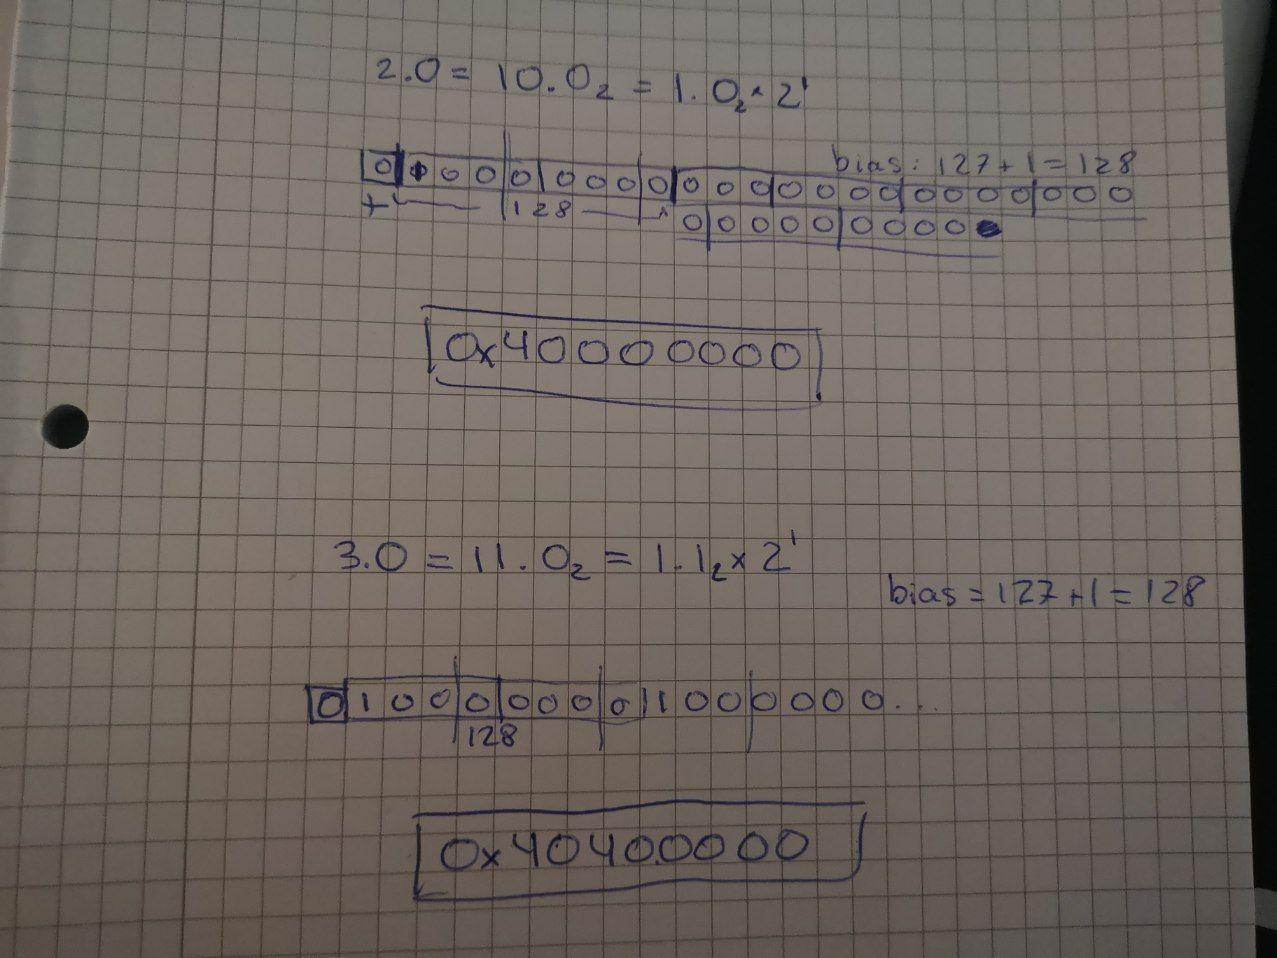
\includegraphics[width=1.0\textwidth]{2and3.jpg}

	\end{answer}

	\pagebreak

	\begin{problem}

    	Oversett 0.50390625 til IEEE 754 32-biter flyttall.

		Legg sammen tallene 2.0 og 0.50390625 med samme fremgangsmåte som Figur 5.30 (du trenger ikke å ta hensyn til avrunding).

	\end{problem}

	\begin{answer}
		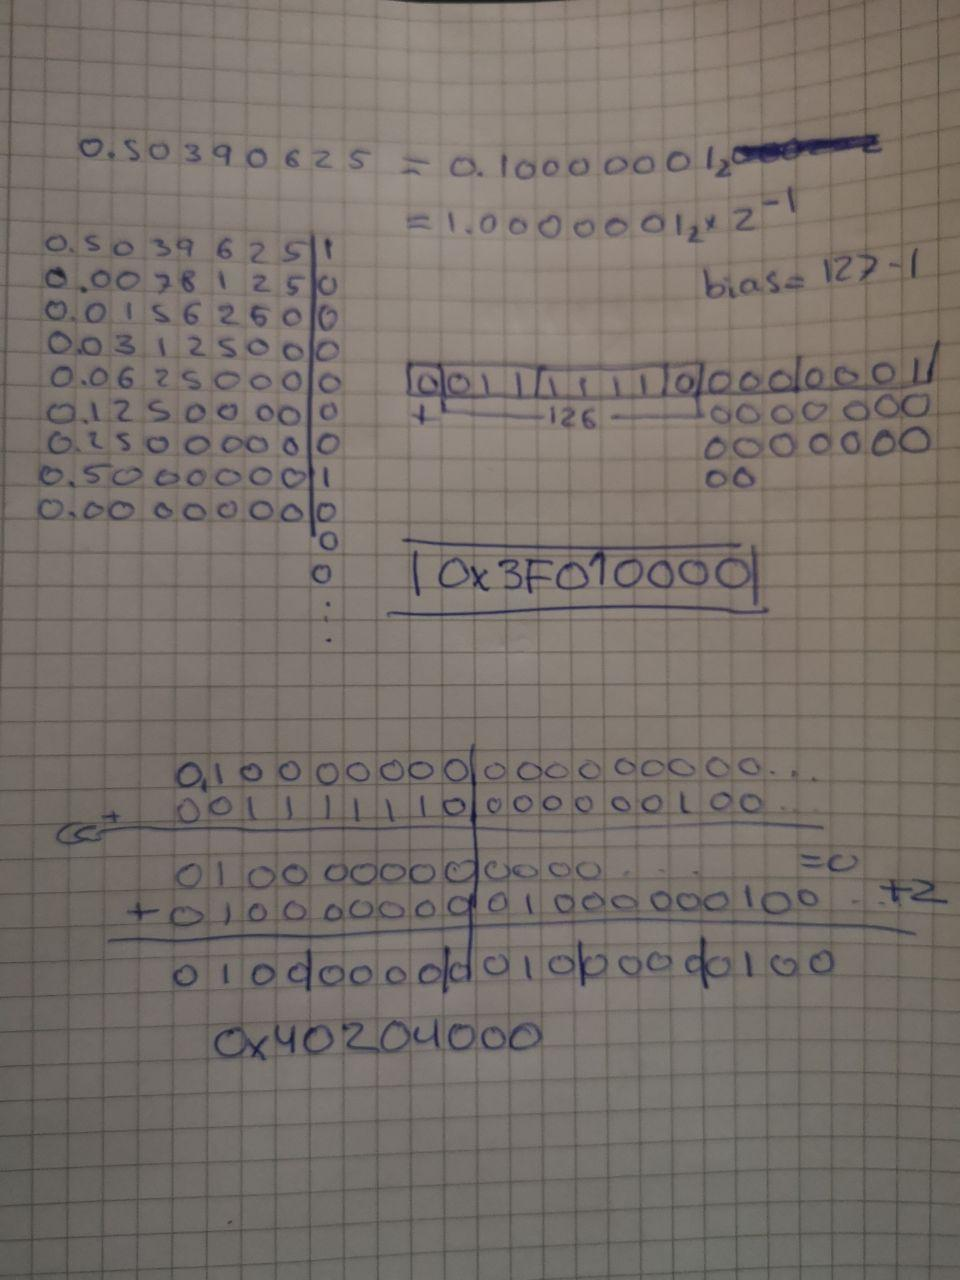
\includegraphics[width=0.8\textwidth]{weirdandsumm.jpg}

	\end{answer}
\end{document}